
\subsection{Classi Principali}

In figura~\ref{fig:classi-principali} sono illustrati i package e le classi principali del sistema di HBS, come definite sopra.

\begin{figure*}[h]
    \centering
    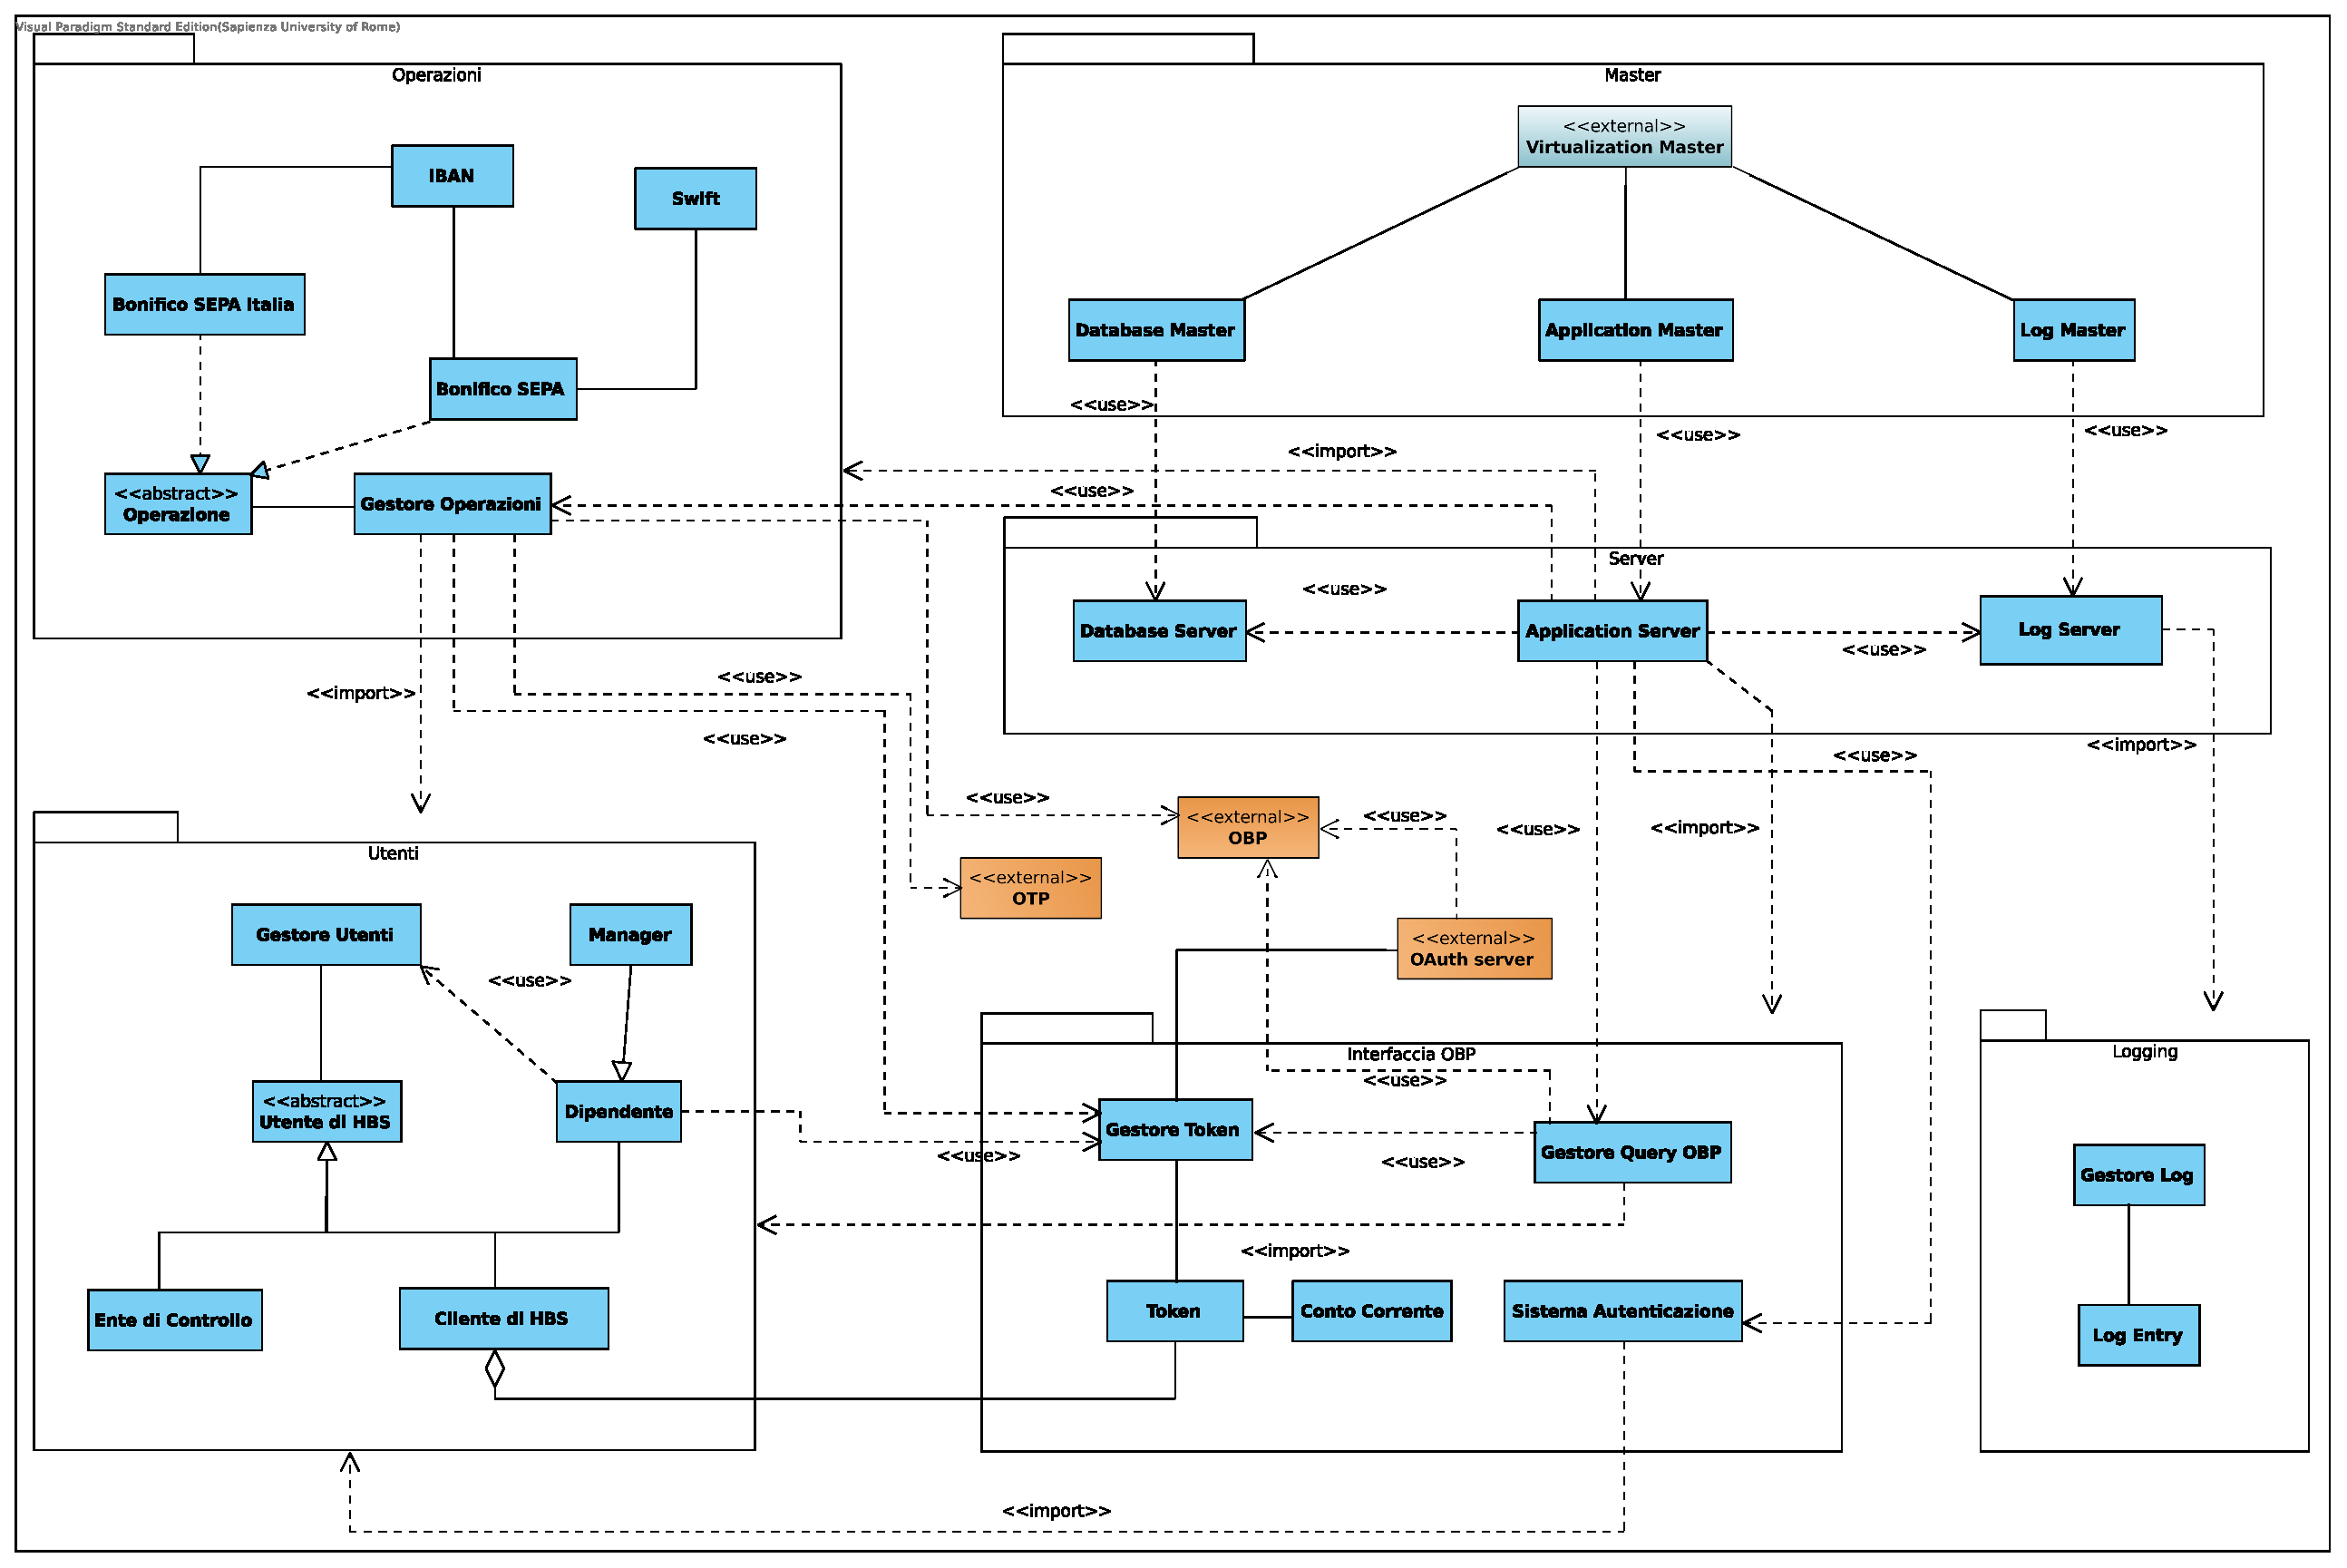
\includegraphics[width=\textheight, angle=90]{Images/Classi_Design.eps}
    \caption{Diagramma delle classi di design di HBS, ristretto alle classi principali.}
    \label{fig:classi-principali}
\end{figure*}

In figura~\ref{fig:classi-principali:operazioni} sono illustrate nel dettaglio le classi del package relativo alle operazioni.

\begin{figure*}[h]
    \centering
    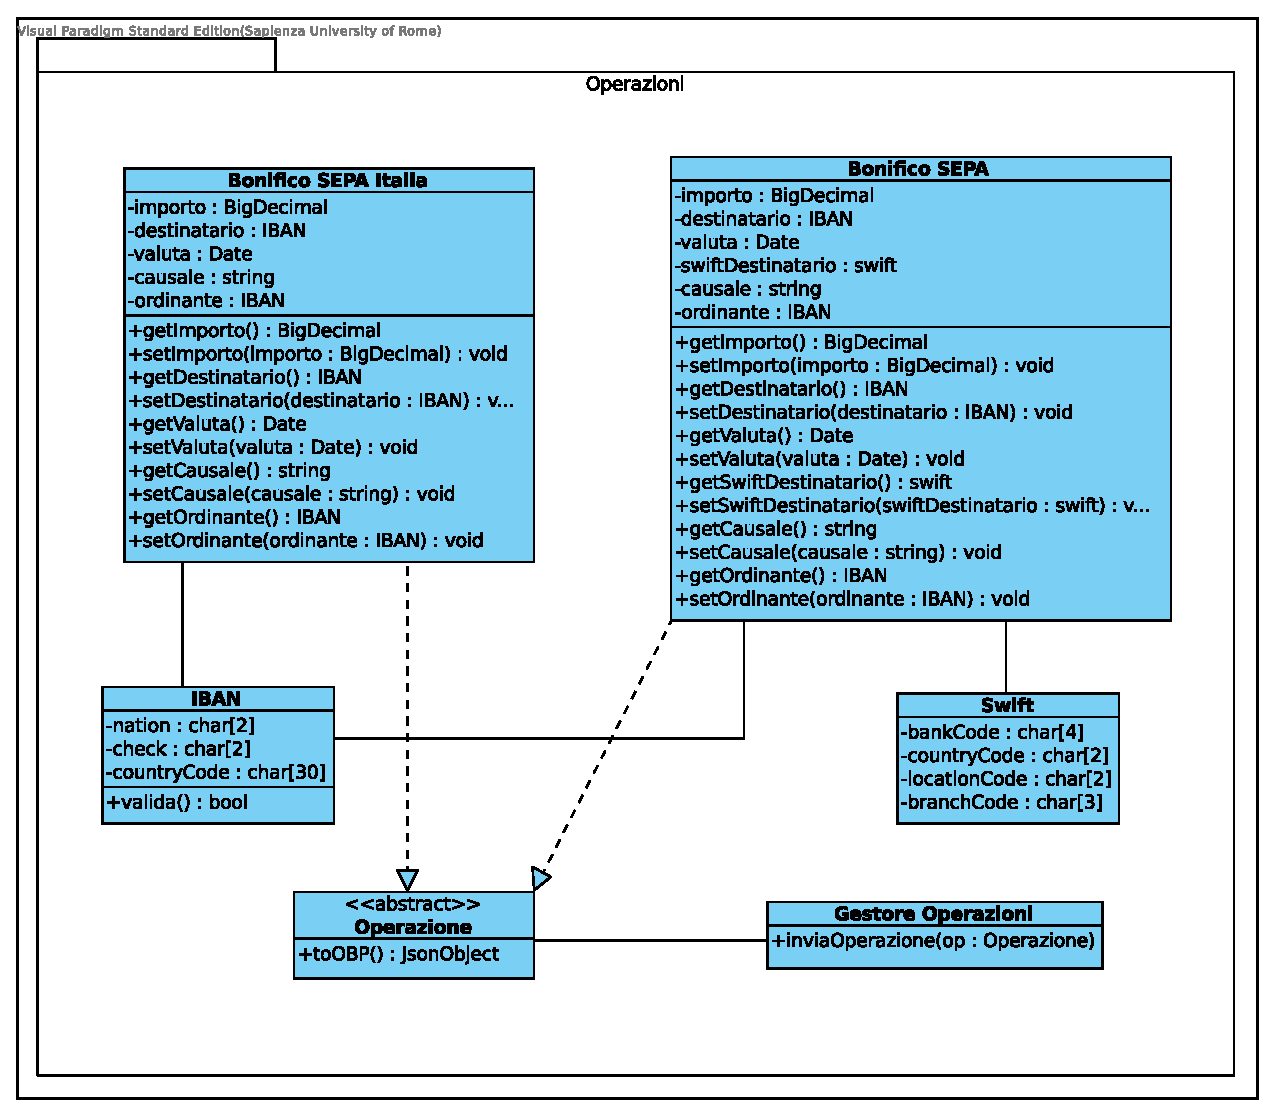
\includegraphics[width=\textwidth]{Images/Operazioni_Design.eps}
    \caption{Diagramma delle classi relative alle operazioni del sistema HBS.}
    \label{fig:classi-principali:operazioni}
\end{figure*}





